% id: 76-31
% book: 쎈B 대수 · 06 삼각함수의 그래프
% section: 유형 07 삼각함수의 그래프의 대칭성
% figure: tikz:fig-76-31
% answer: 
% answer_source: 
% variant_level: 0 (원본 전사)
% 이 파일은 build.mjs 가 items.json 에서 만든다. 고칠 때는 items.json 을 고친다.
다음 그림과 같이 함수 $f(x)=\cos kx\left(0\le x\le\dfrac{5\pi}{2k}\right)$의 그래프와 직선 $y=\dfrac{3}{4}$이 세 점 $\pt{A}$, $\pt{B}$, $\pt{C}$에서 만난다. 세 점 $\pt{A}$, $\pt{B}$, $\pt{C}$의 $x$좌표를 각각 $\alpha$, $\beta$, $\gamma$라 할 때, $f(2\alpha+2\beta-\gamma)$의 값을 구하시오. \dmcondfill{$k$는 양수이고, $\alpha<\beta<\gamma$이다.}{}
\par\smallskip\begin{center}\resizebox{\ifdim\width>\linewidth\linewidth\else\width\fi}{!}{% 76-31(76쪽) — $f(x)=\cos kx\ \left(0\le x\le\dfrac{5\pi}{2k}\right)$ 의 그래프와 직선 $y=\dfrac{3}{4}$(원문 「다음 그림」 · 본문 아래 전폭).
% 스캔 화질이 낮아 TikZ 로 다시 그림. 라벨은 원문 것만: $y$축의 $1$, 세 교점 A·B·C 와 $x$좌표 $\alpha$·$\beta$·$\gamma$,
% 오른쪽 끝 $\dfrac{5\pi}{2k}$, $\pt{O}$, 직선 이름 $y=\dfrac{3}{4}$, 곡선 이름 $y=f(x)$. $x$ 한 칸은 $\dfrac{\pi}{k}$.
% $f(2\alpha+2\beta-\gamma)$ 의 값(답)이 읽히지 않게 $x$축 눈금은 적지 않는다.
\begin{tikzpicture}[line width=0.6pt, x=1.36cm, y=0.53cm, >=stealth]
  \draw[densely dashed, line width=0.35pt] (0.23,0) -- (0.23,0.75);
  \draw[densely dashed, line width=0.35pt] (1.77,0) -- (1.77,0.75);
  \draw[densely dashed, line width=0.35pt] (2.23,0) -- (2.23,0.75);
  \draw[line width=0.55pt] (-0.22,0.75) -- (2.78,0.75);
  \draw[->, line width=0.7pt] (-0.22,0) -- (2.86,0);
  \draw[->, line width=0.7pt] (0,-1.5) -- (0,1.5) node[left=1pt, font=\small] {$y$};
  \draw[domain=0:2.5, samples=160, smooth] plot (\x, {cos(180*\x)});
  \fill (0,1) circle (2.2pt);
  \fill (2.5,0) circle (2.2pt);
  \node[font=\small, anchor=east] at (-0.05,1) {$1$};
  \node[font=\small, anchor=south west] at (0.25,0.80) {$\pt{A}$};
  \node[font=\small, anchor=south] at (1.74,0.80) {$\pt{B}$};
  \node[font=\small, anchor=south] at (2.20,0.80) {$\pt{C}$};
  \node[font=\small, anchor=north] at (0.23,-0.06) {$\alpha$};
  \node[font=\small, anchor=north] at (1.77,-0.06) {$\beta$};
  \node[font=\small, anchor=north east] at (2.27,-0.06) {$\gamma$};
  \node[font=\small, anchor=north] at (2.58,-0.10) {$\dfrac{5\pi}{2k}$};
  \node[font=\small, anchor=north east] at (-0.04,-0.04) {$\pt{O}$};
  \node[font=\small, anchor=north] at (2.83,-0.06) {$x$};
  \node[font=\small, anchor=west] at (2.90,0.75) {$y=\dfrac{3}{4}$};
  \node[font=\small, anchor=north west] at (0.92,-0.95) {$y=f(x)$};
\end{tikzpicture}
}\end{center}
